\chapter{UML models}

\section{Use cases}
In this section we are going to analyze some of the use cases mentioned in the diagram of the figure~\ref{fig:use_case_diagram} and derived from the scenarios described in chapter~\ref{chap:scenarios} of this document.

\begin{figure}[t]
	\centering
	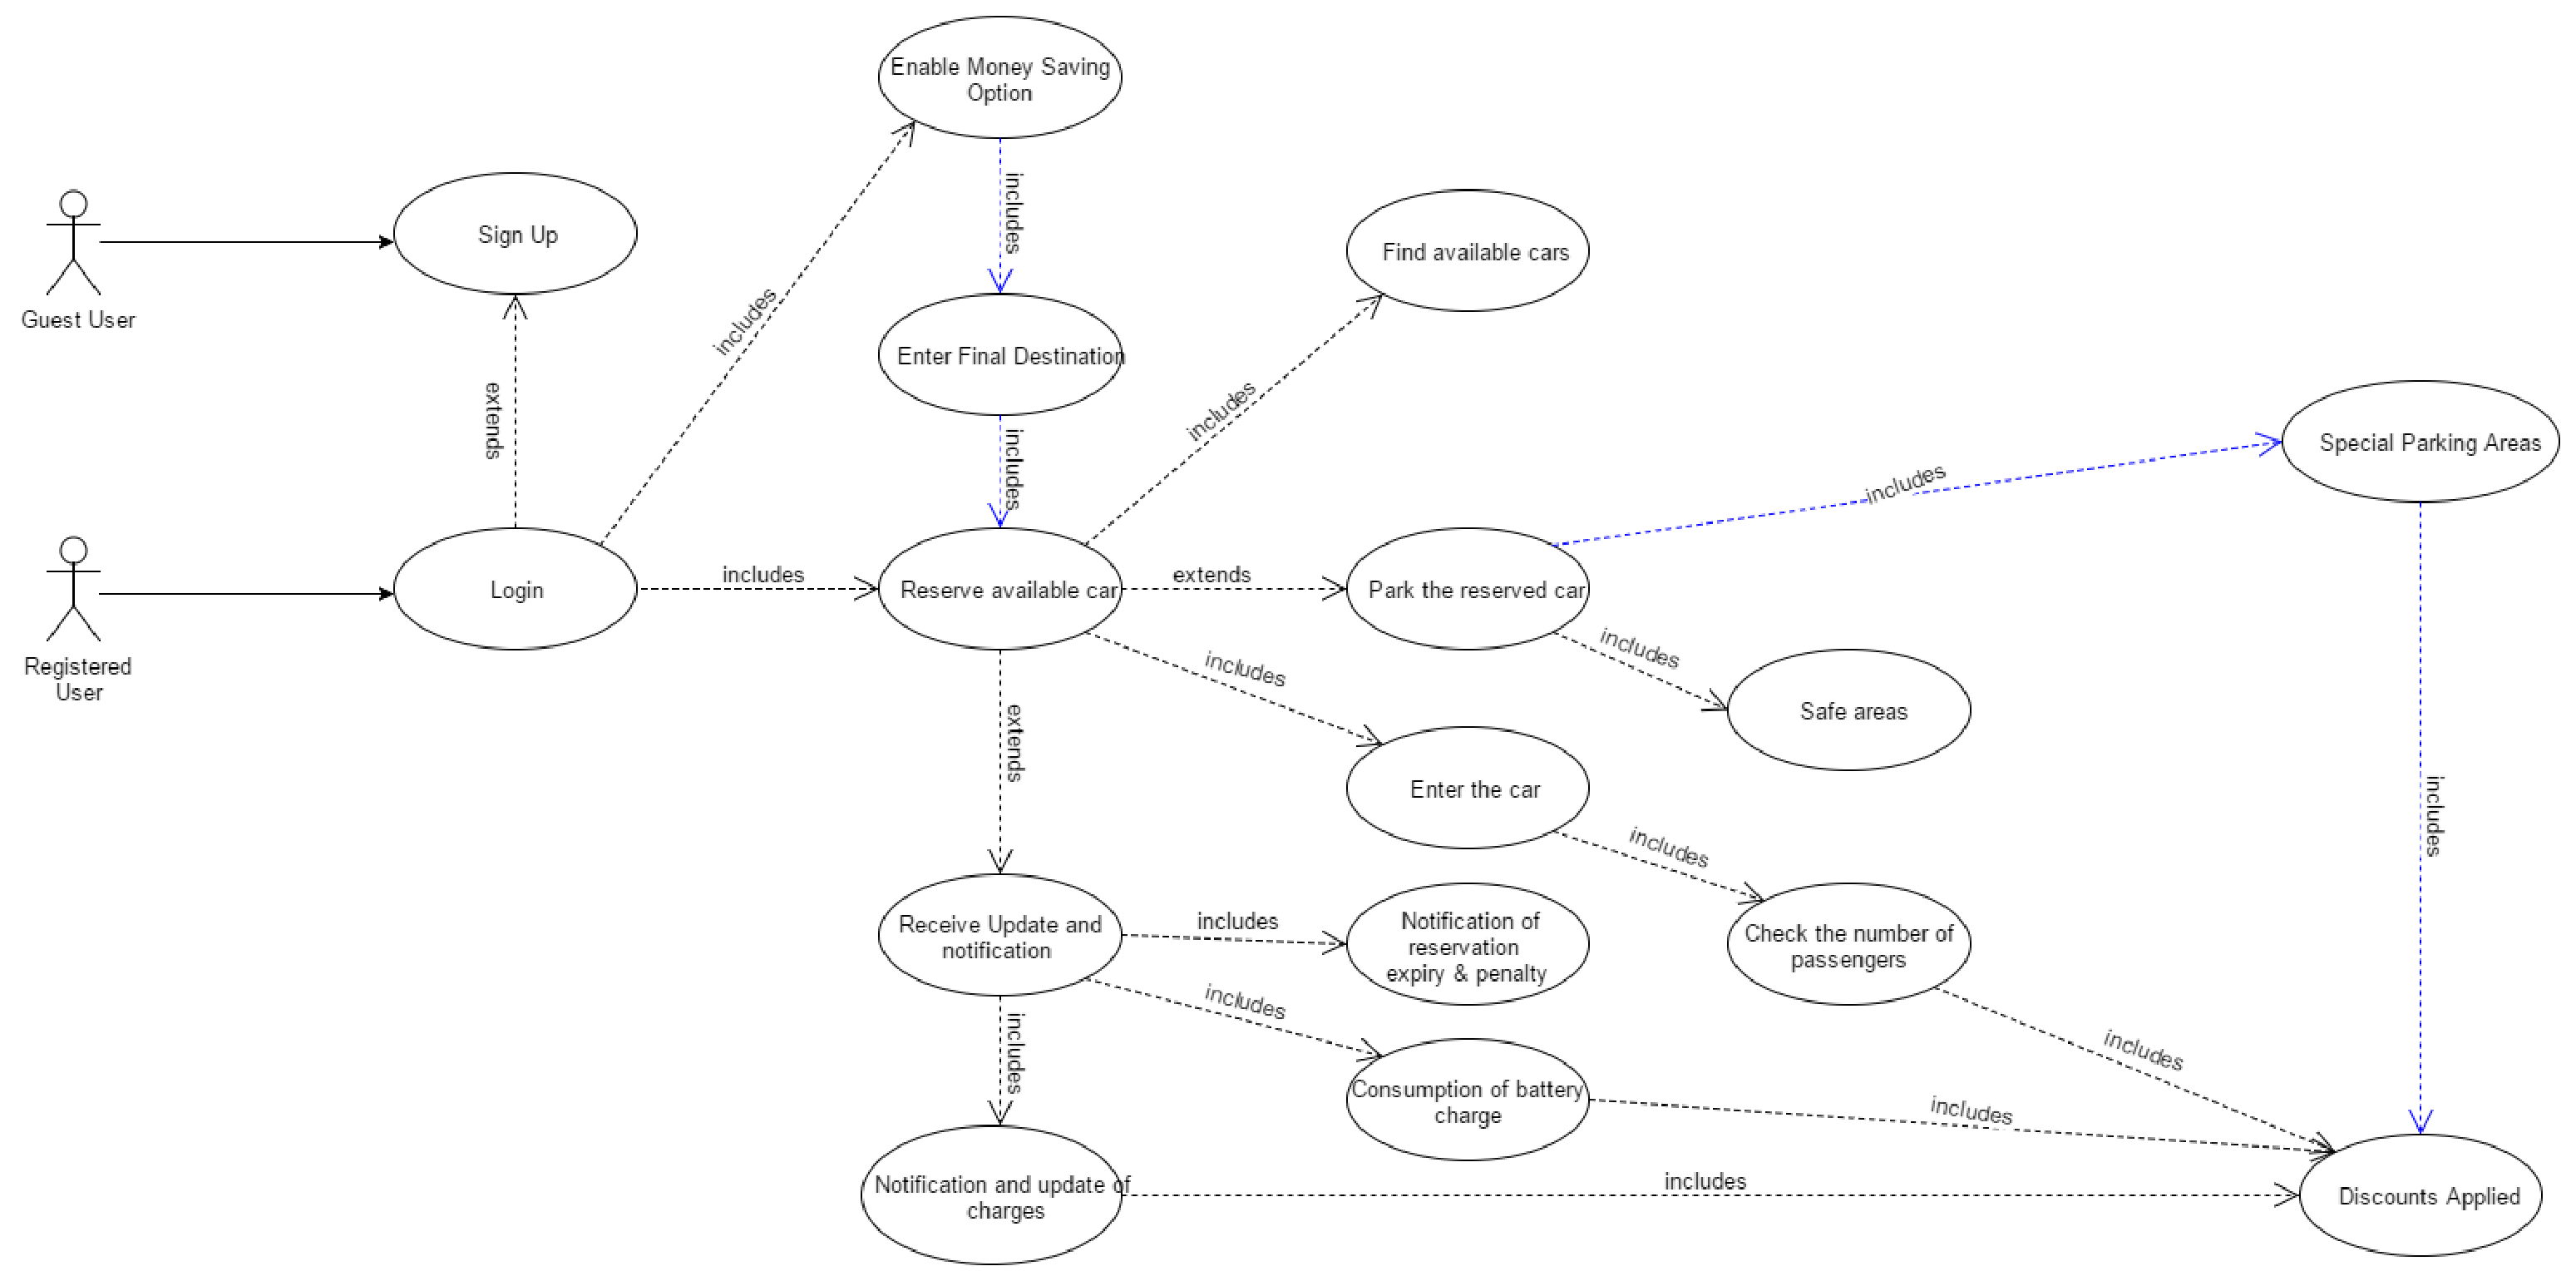
\includegraphics[height=6.7cm,keepaspectratio]{figures/use_case_diagram.eps}
	\caption{Use case diagram for PowerEnJoy}
	\label{fig:use_case_diagram}
\end{figure}

\subsection{Guest sign-up}
\begin{itemize}
	\item \emph{Actors}: Unregistered user
	\item \emph{Entry conditions}: User must not be registered.
	\item \emph{Flow of events}:
	\begin{itemize}
		\item The user arrives at the home page of the mobile app or desktop version.
		\item The user clicks on the Sign Up button.
		\item The user inputs its personal data, including one valid ID and a valid drive license.
		\item The user must confirm the registration browsing a link sent by the system to the email address specified by the user.
		\item The system checks the profile and the input data are validated.
		\item The user must input in the app's homepage the 6 digit code sent by the system to the specified mobile number.
		\item The system validates the account, the user gets notified by sms and notification.
	\end{itemize}
	\item \emph{Exit conditions}: User's account is validated.
	\item \emph{Exceptions}: If the system rejects the input data, the user can find explanations in the app's home page, where he can insert the missing data. If the user doesn't receive the SMS he can ask the app to send it again.
\end{itemize}

\subsection{User login}
\begin{itemize}
	\item \emph{Actors}: Registered user
	\item \emph{Entry conditions}: User must have a confirmed account.
	\item \emph{Flow of events}:
	\begin{itemize}
		\item The user arrives at the homepage of the mobile app or desktop version.
		\item The user inputs its credentials in the drop-down menu.
		\item The user clicks on login.
		\item The user is redirected to his personal page.
	\end{itemize}
	\item \emph{Exit conditions}: The user is successfully redirected to his personal page.
	\item \emph{Exceptions}: The credentials specified by the user were wrong. The user is notified and he can input them again.
\end{itemize}

\subsection{User reserves an available car}
\begin{itemize}
	\item \emph{Actors}: Registered user
	\item \emph{Entry conditions}: User must have a validated account and be logged in.
	\item \emph{Flow of events}:
	\begin{itemize}
		\item The user arrives at his personal page of the mobile app or desktop version.
		\item The user clicks on Find Available Car to full size the map.
		\item The user selects a car and clicks Reserve.
		\item The user is notified with both SMS and app notification about the reservation and the instructions to abort it.
		\item The user approaches the car.
		\item The user asks the system to unlock the car.
		\item The system checks the user's position through the GPS.
		\item If the user's GPS position matches with the car's one, the car is unlocked.
		\item The user can specify whether to enable the Money Saving Option and the destination (mandatory if this option is enabled).
		\item The user ignites the engine and the system starts charging.
		\item The system takes notes about the number of passengers.
		\item The user drive to his destination.
		\item If the Money Saving Option is enabled, the system suggests the user the special parking area where to park.
		\item The user looks for an available parking spot, while verifying on the app's map that it's not forbidden by the service's policies.
		\item The user parks the car.
		\item The user stops the engine and the system stops charging.
		\item The user leaves the car.
		\item If the parking area isn't forbidden the car gets locked by the system, otherwise the user will be asked to get back in the car and change parking spot.
		\item The system checks the battery status, the distance between the parking slot and the closest power station grid, and along with the previously acquired number of passengers, it applies penalties and discount according to the terms and conditions.
		\item The user gets notified about the final charge along with the discounts.
	\end{itemize}
	\item \emph{Exit conditions}: The user gets notified by the system and the car is locked.
	\item \emph{Exceptions}: If the GPS positions of the car and the user don't match, the user is notified to get closer to the car. If the user parks in a low GPS coverage area, the system will notify the user in time. The same if the user parks in a non-safe area. If the user doesn't get back in the car within X minutes, the car gets locked and the user gets penalties.
\end{itemize}

\newpage
\section{Sequence diagrams}

\subsection{Registration of a user}
\begin{figure}[h]
	\centering
	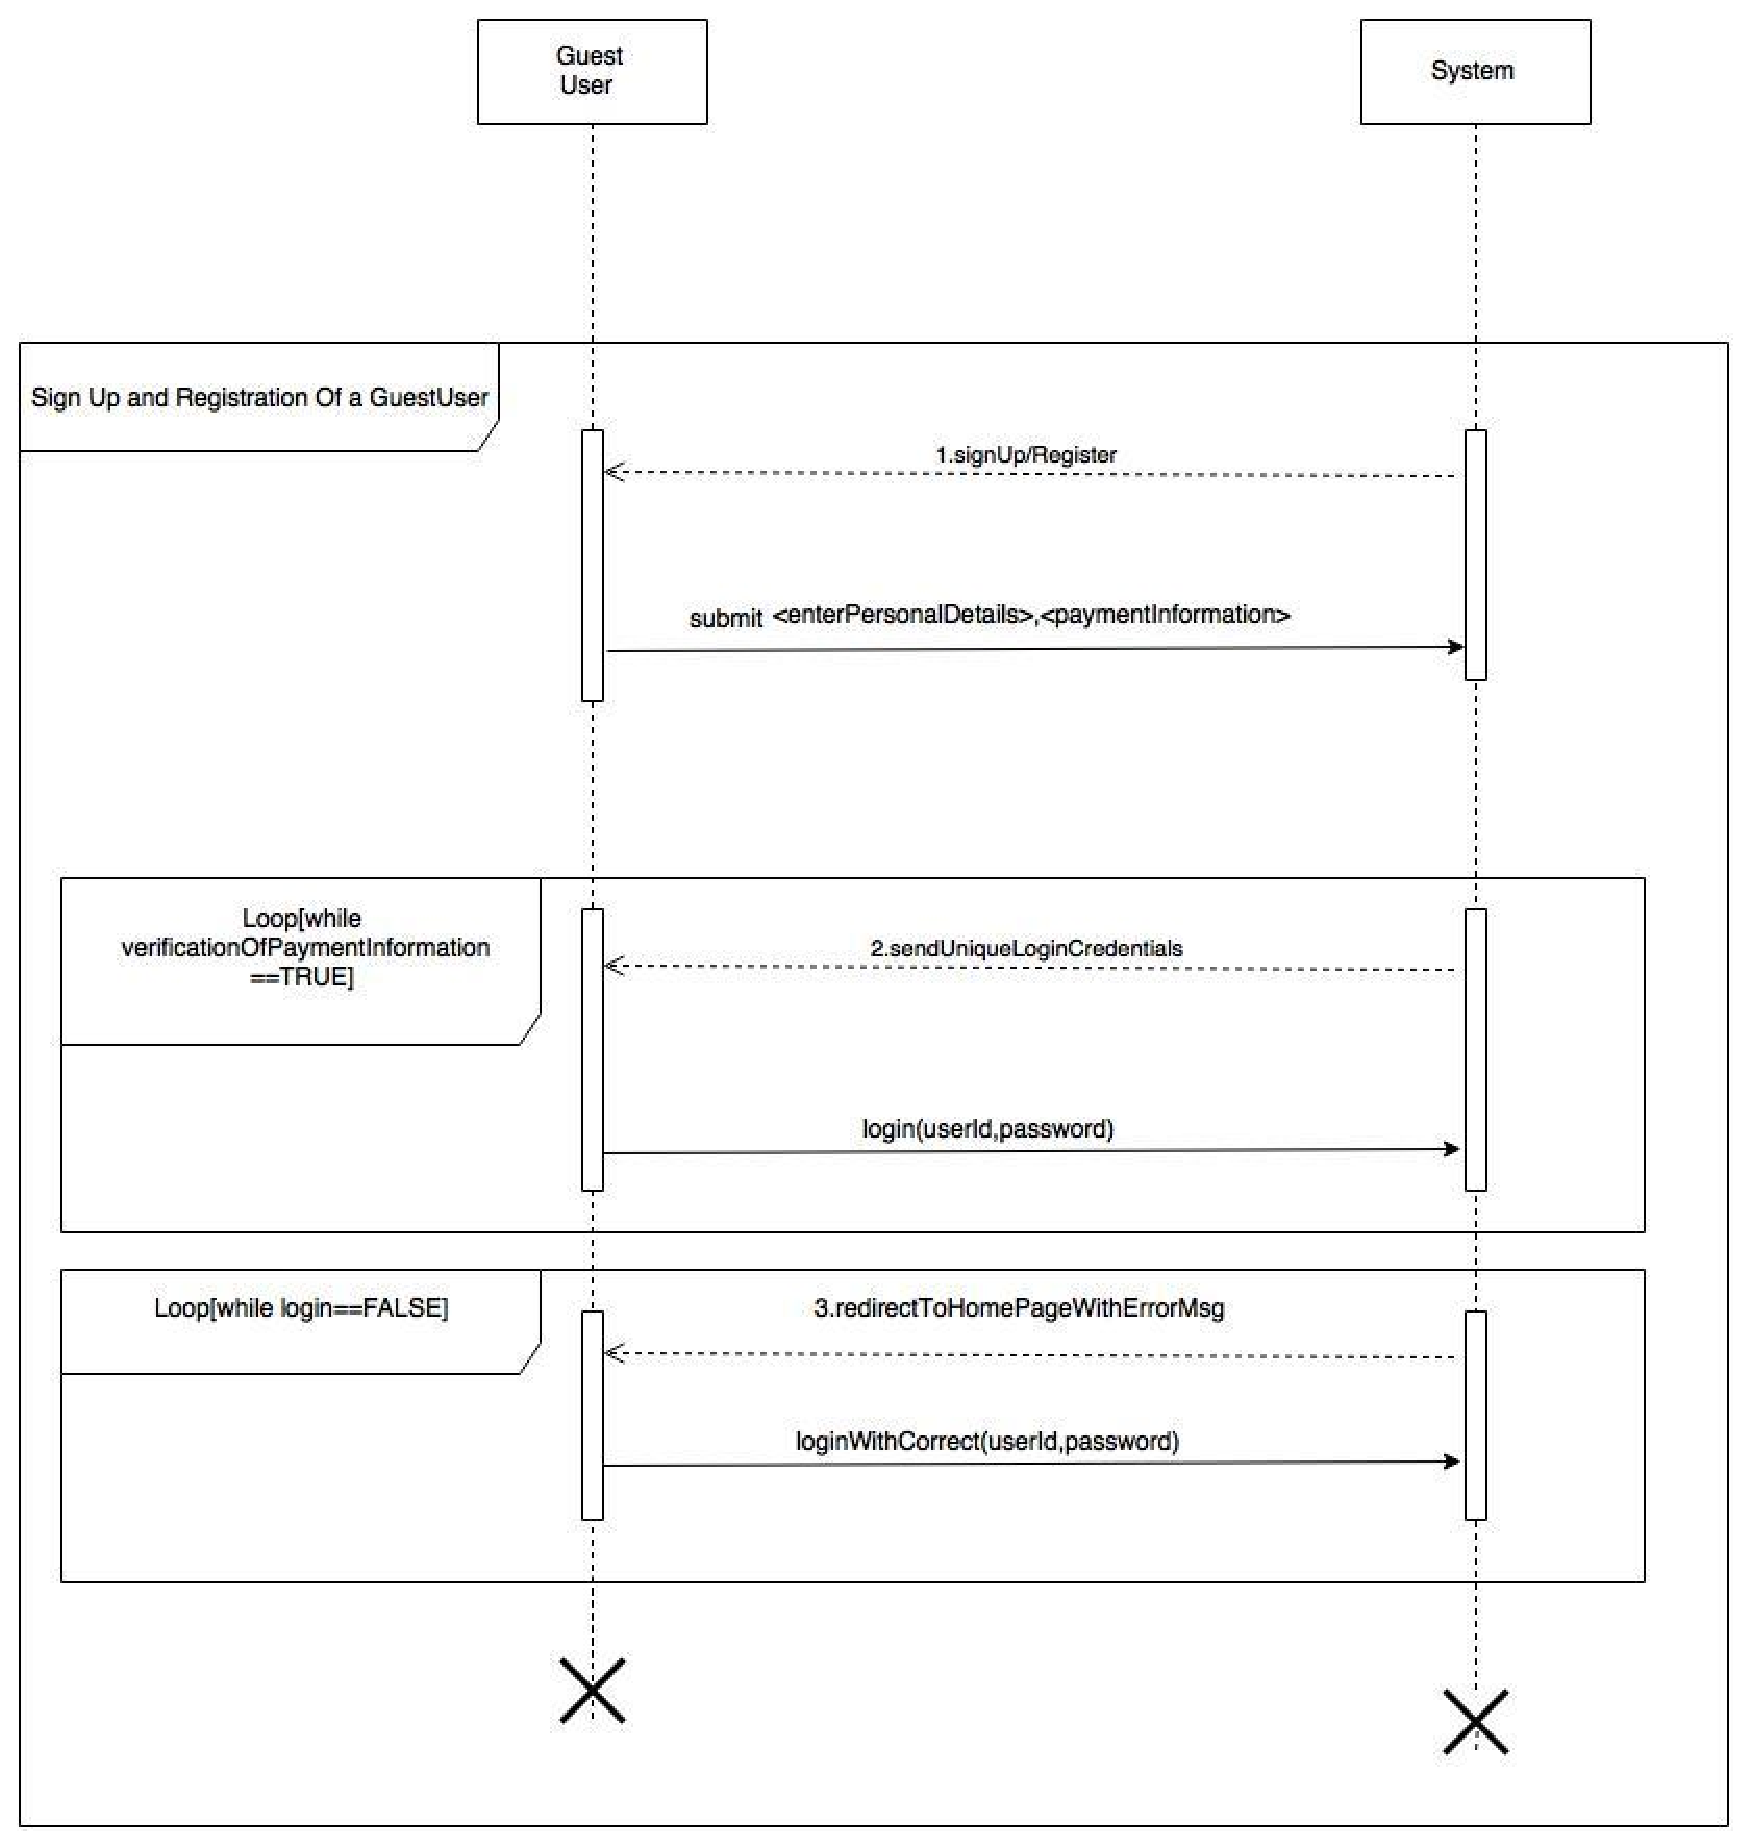
\includegraphics[height=15.2cm,keepaspectratio]{figures/sequence_register.eps}
	\caption{Sequence diagram for the registration of a user}
	\label{fig:sequence_register}
\end{figure}

\newpage
\subsection{Reservation of a car}
\begin{figure}[h]
\centering
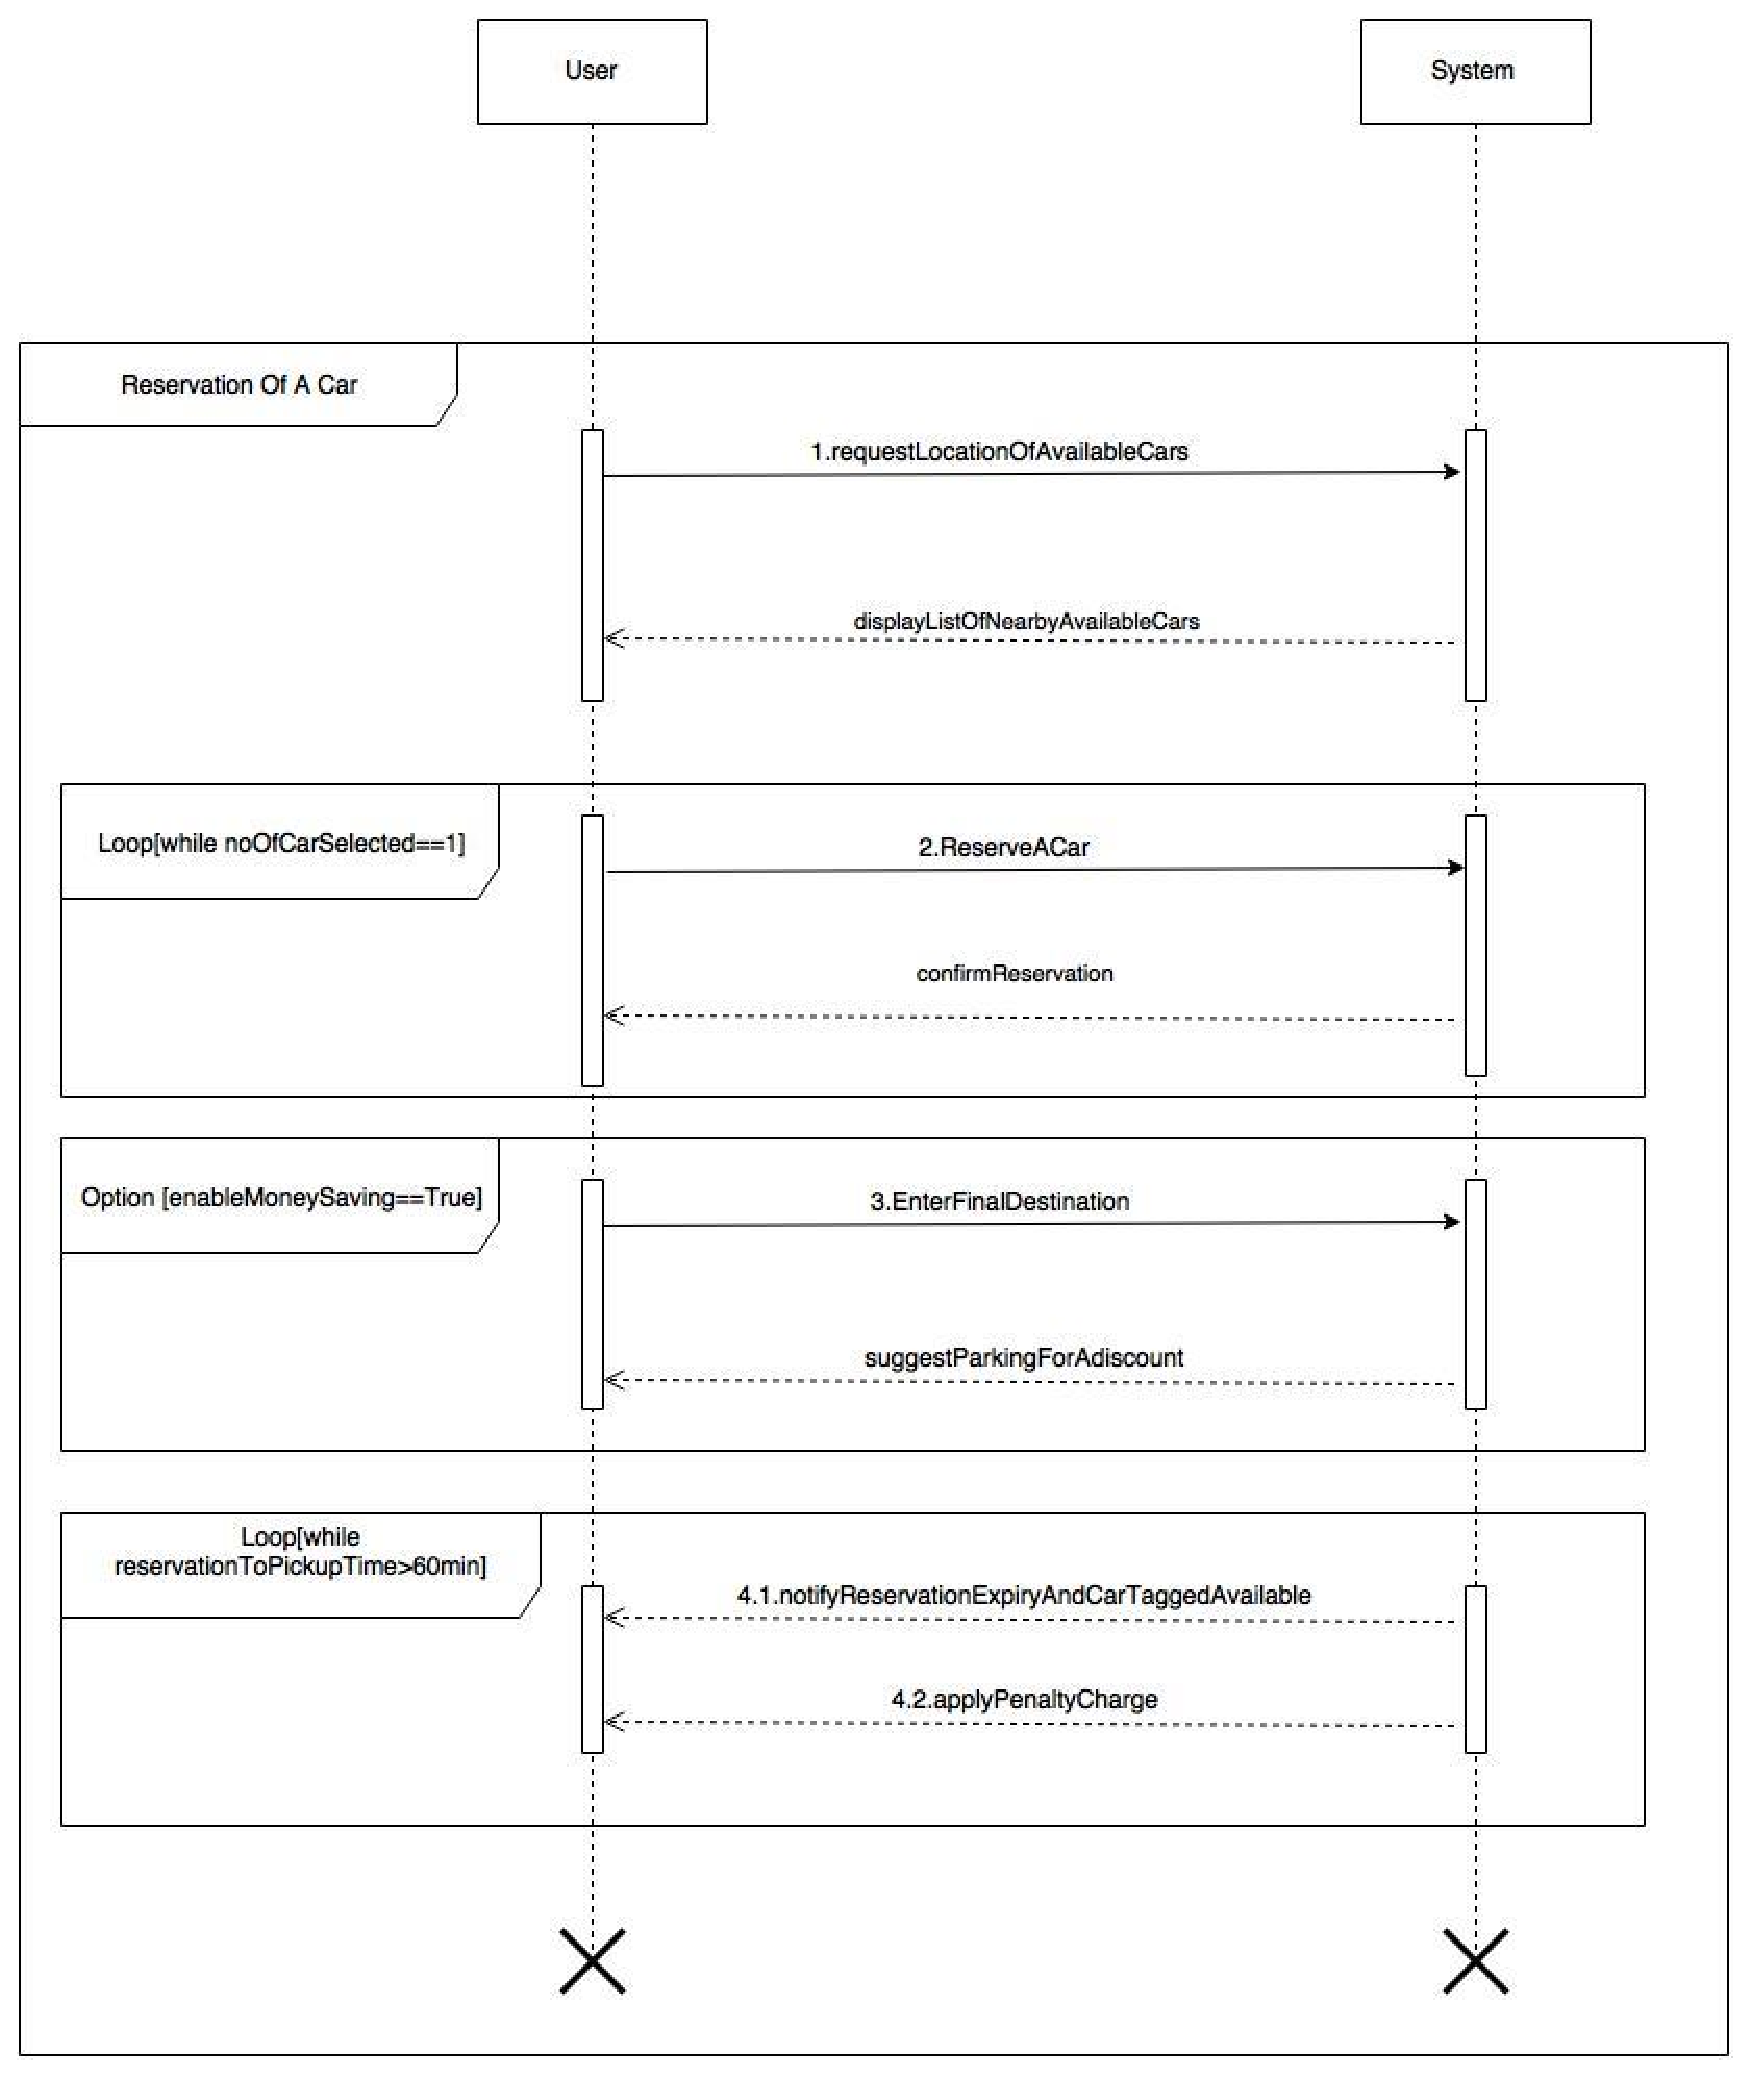
\includegraphics[height=15.2cm,keepaspectratio]{figures/sequence_reservation.eps}
\caption{Sequence diagram for the reservation of a car}
\label{fig:sequence_reservation}
\end{figure}

\newpage
\subsection{Discounts and penalties}
\begin{figure}[h]
\centering
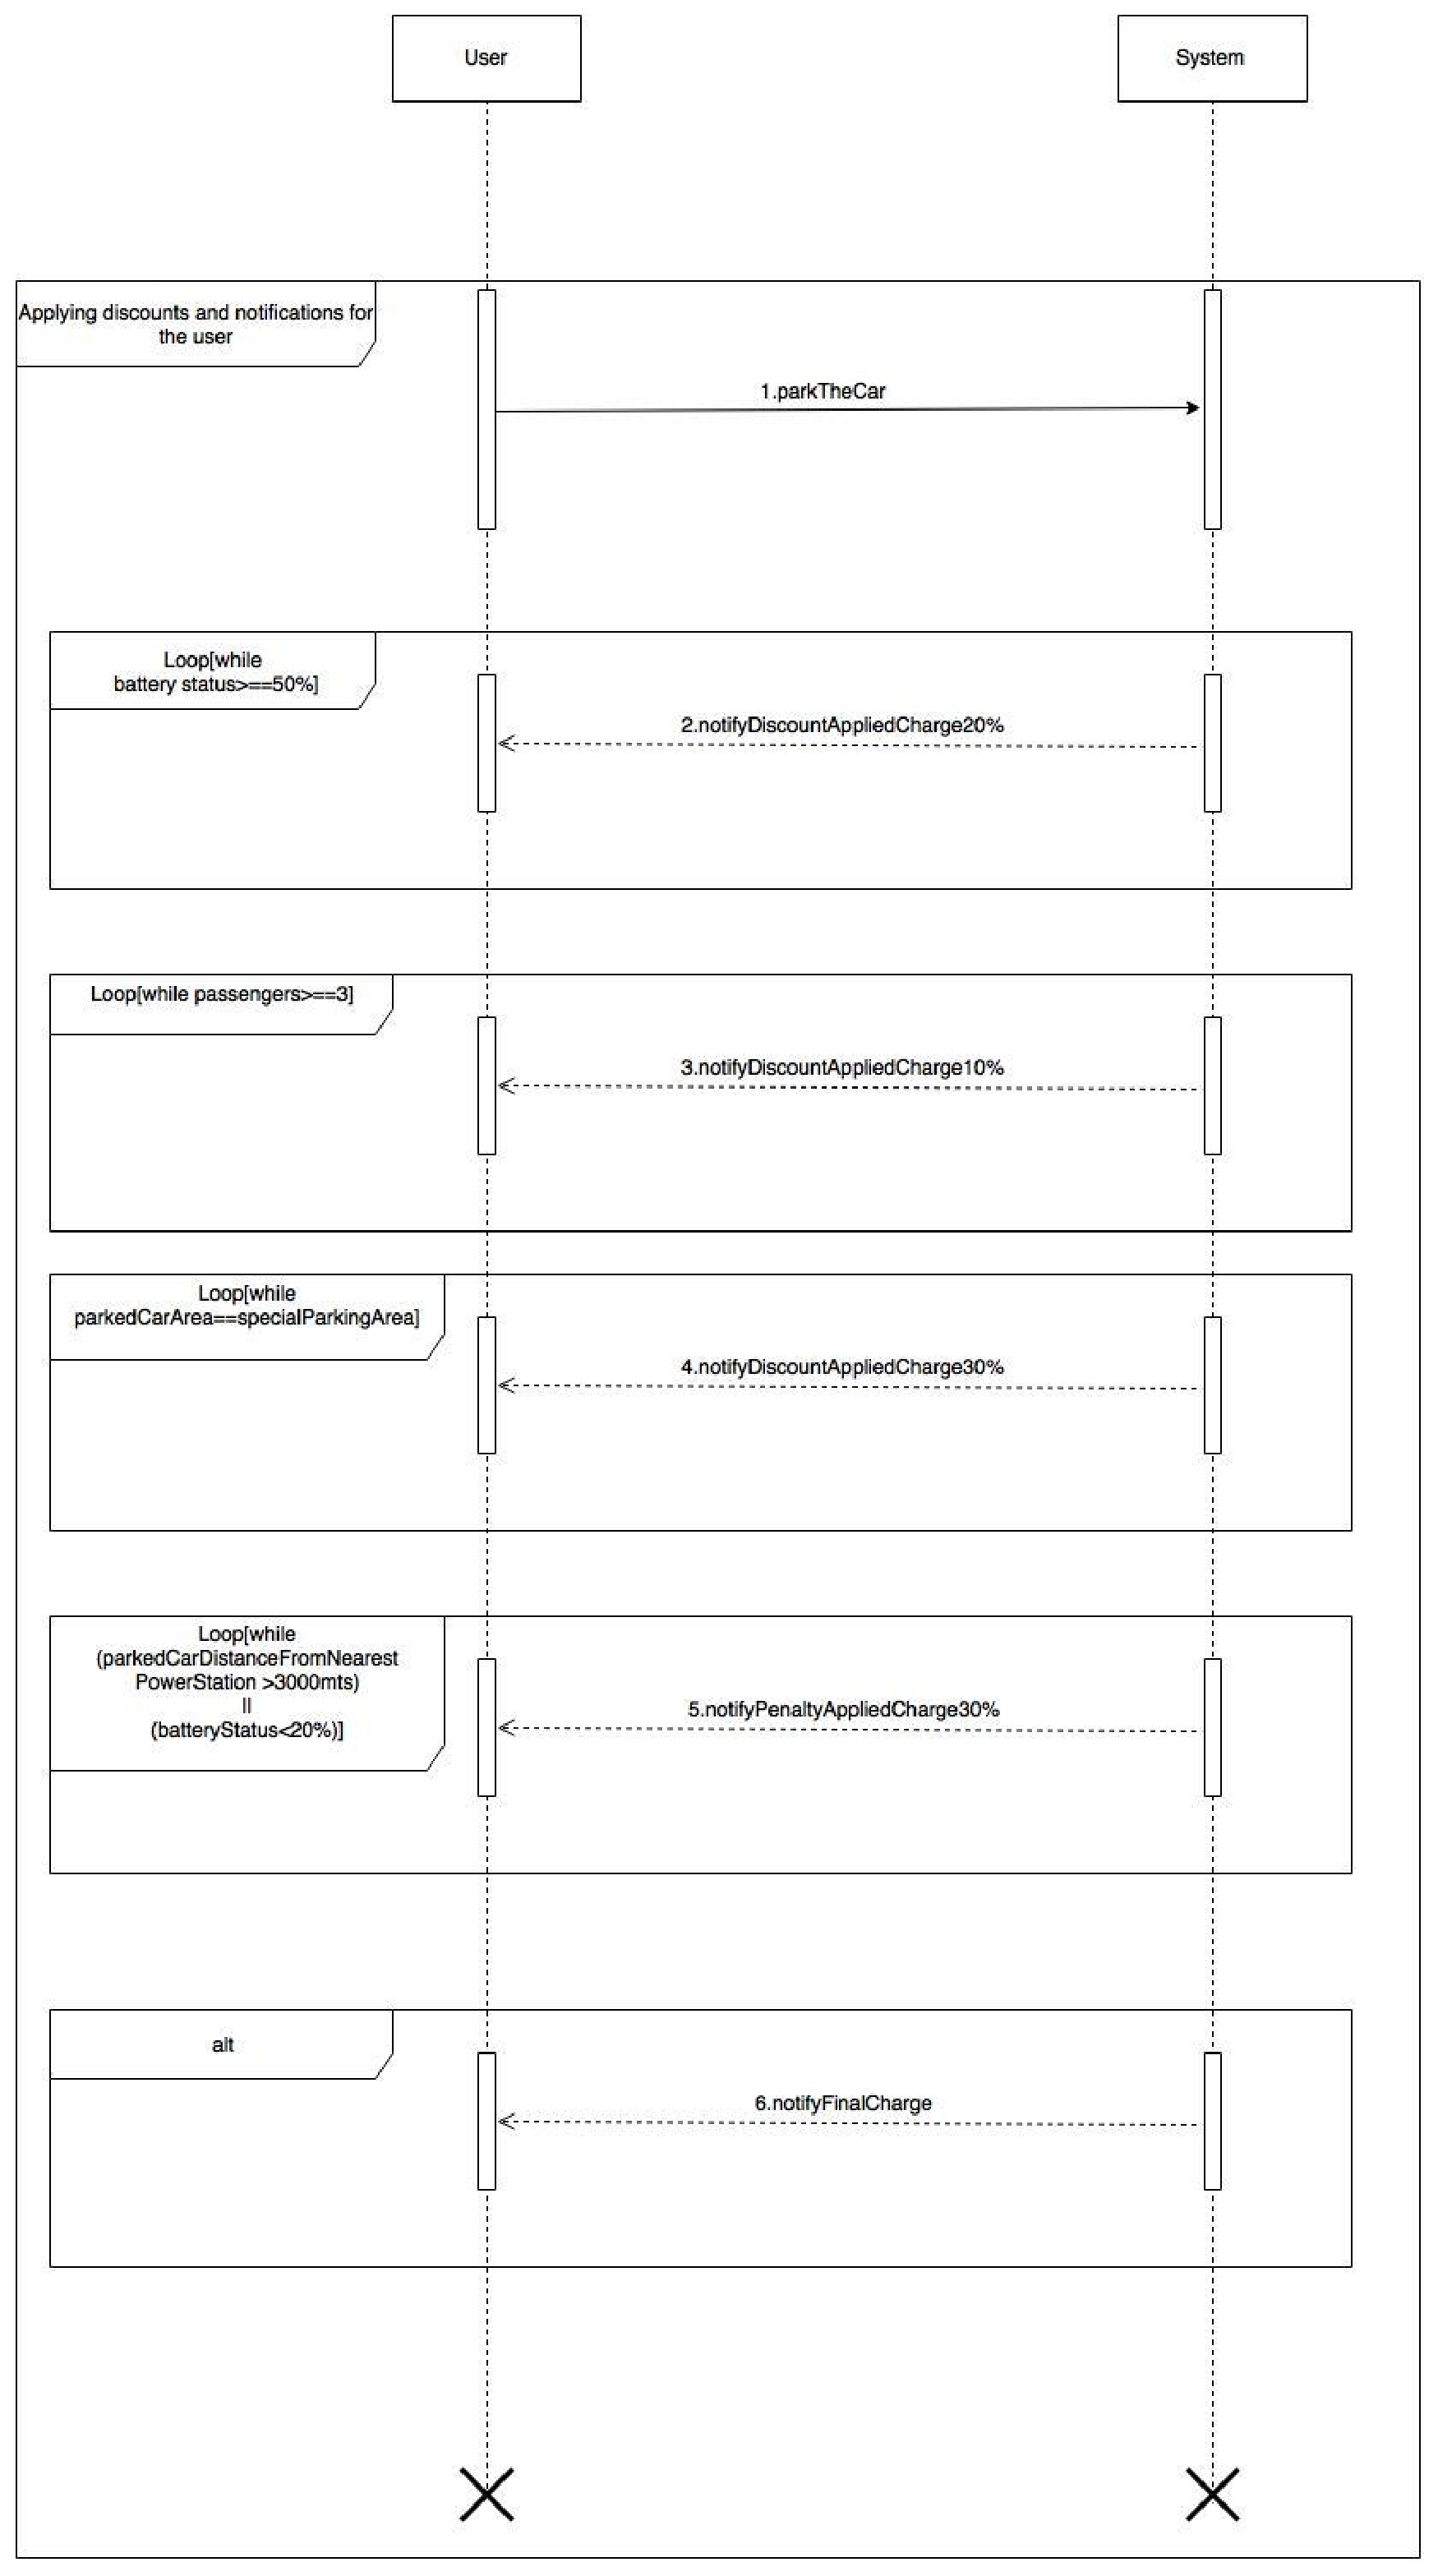
\includegraphics[height=15.2cm,keepaspectratio]{figures/sequence_discounts_penalties.eps}
\caption{Sequence diagram for the application of discounts and penalties}
\label{fig:sequence_discounts_penalties}
\end{figure}

\newpage
\section{Class diagram}
\begin{figure}[h]
	\centering
	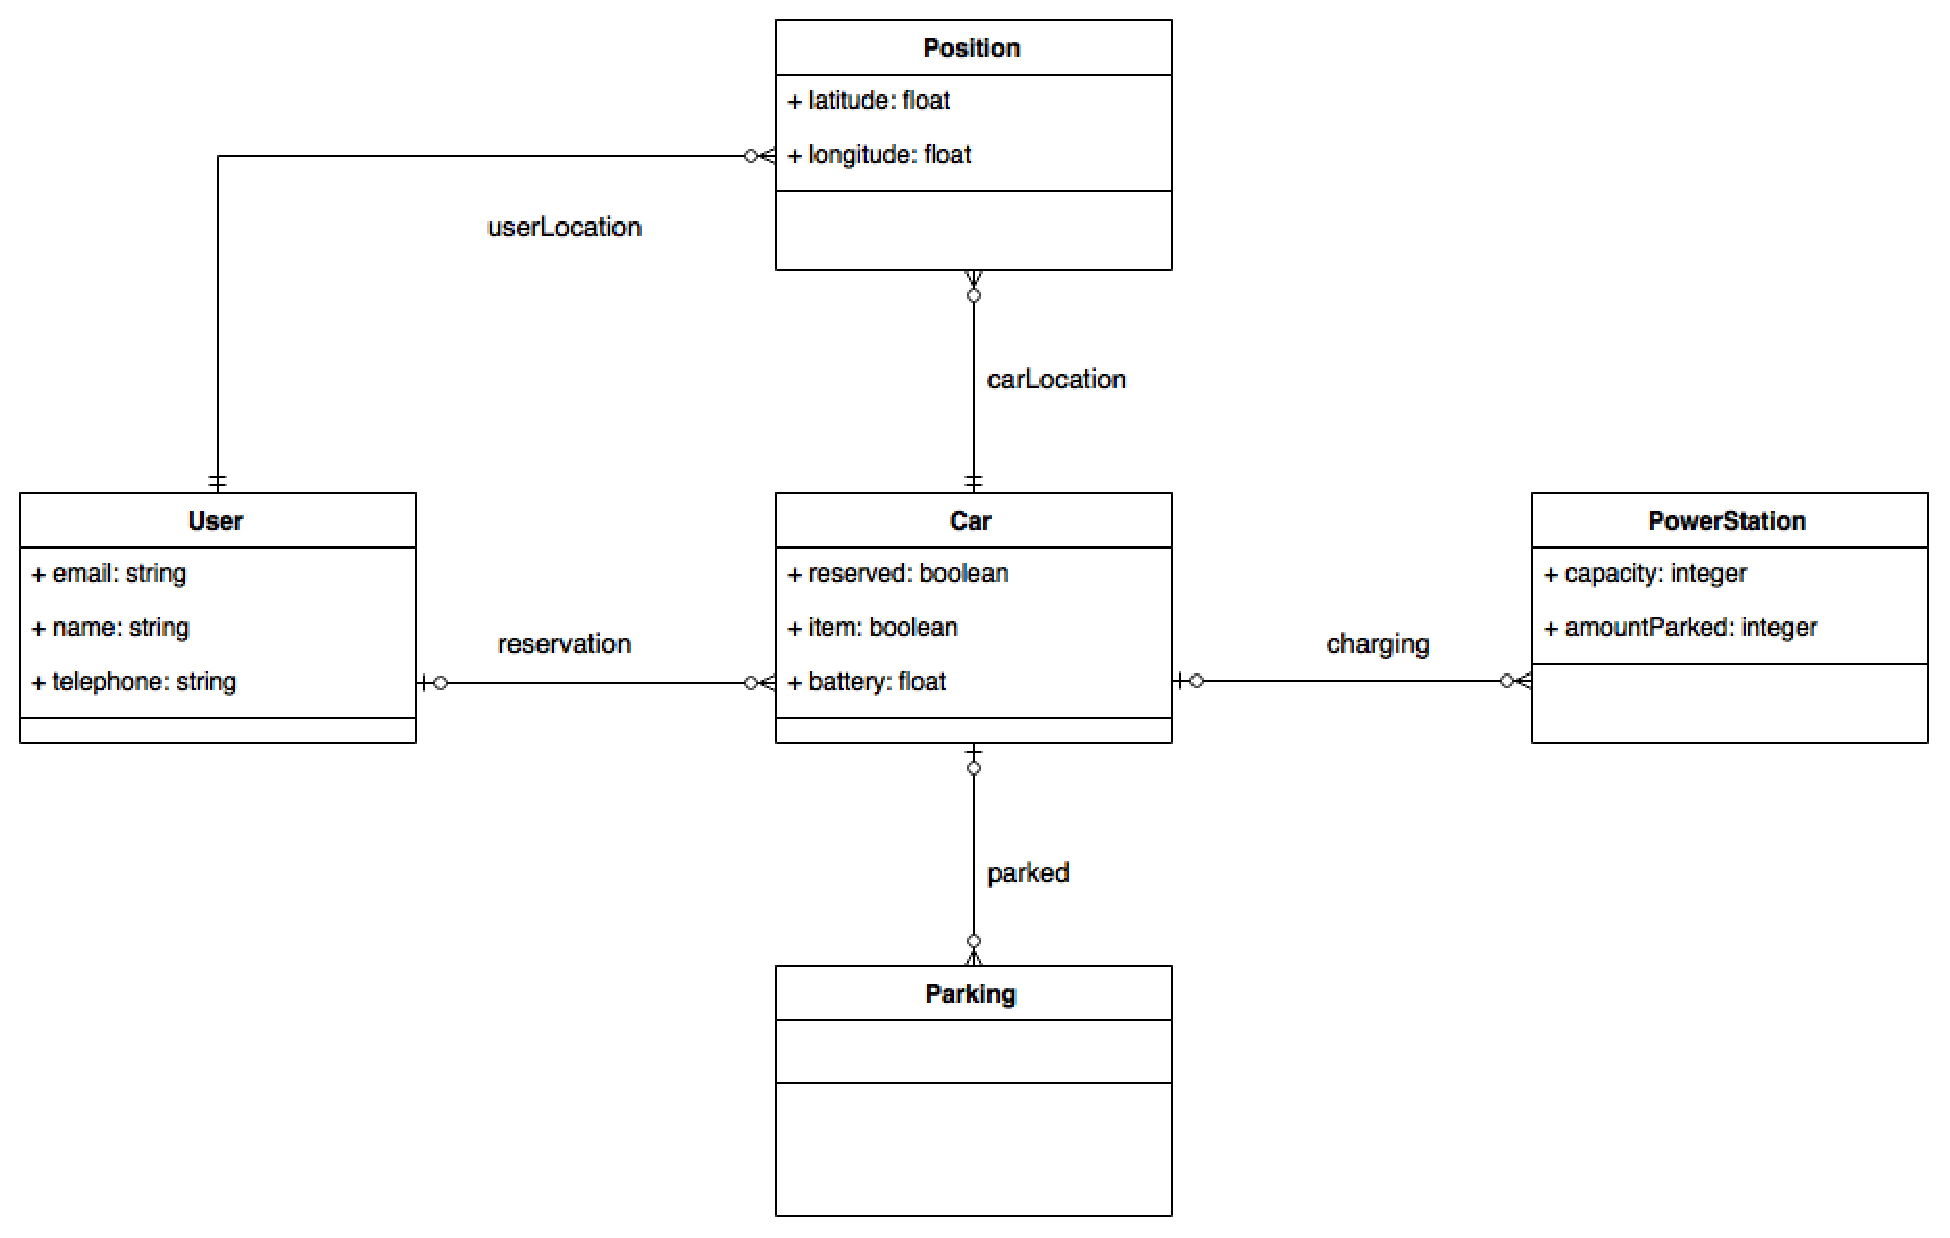
\includegraphics[width=\textwidth,keepaspectratio]{figures/class_diagram.eps}
	\caption{Class diagram for PowerEnJoy}
	\label{fig:class_diagram}
\end{figure}